\chapter{Accenni di fisica del neutrino}
\label{cap:Neutrino}
I neutrini, dopo i fotoni, sono le particelle più abbondanti in tutto l'Universo. Ogni secondo, decine di miliardi di neutrini attraversano ogni centimetro quadrato del nostro corpo, eppure dalla prima ipotesi della loro esistenza, formulata da W. Pauli, sono trascorsi molti anni prima di ottenere una conferma sperimentale. Nel Modello Standard delle particelle elementari, i neutrini sono classificati come fermioni appartenenti alla famiglia dei leptoni, elettricamente neutri e inizialmente considerati privi di massa. Poiché possono interagire solo tramite l'interazione debole, i neutrini risultano particolarmente difficili da rilevare. Tuttavia, grazie a numerosi esperimenti volti a esplorare la loro natura, è stata scoperta l'evidenza di un nuovo fenomeno fisico: l'oscillazione dei neutrini.%neutrino physics and astrophysics overview
%citare pauli: I have done something very bad today by proposing a particle that cannot be detected; it is something no theorist should ever do. - Wolfgang Pauli

\section{Ipotesi dell'esistenza del neutrino}
I risultati che sono emersi dai primi studi dello spettro energetico dell'elettrone in un decadimento $\beta$, ha portato, come prima ipotesi che un'interazione di questo tipo potesse violare la conservazione dell'energia. Inizialmente si pensava che il decadimento $\beta$ fosse un processo a due corpi, descrivibile tramite la reazione \ref{eq:prevbeta}
\begin{equation}
    \beta:\quad \ce{^A_ZX}\longrightarrow \ce{^A_{Z+1}Y}\,+\,e^-
    \label{eq:prevbeta}
\end{equation}
dove $Y$ è il nucleo in cui un neutrone si è trasformato in un protone e $e^-$ rappresenta l'elettrone emesso.
In questo tipo di processo, la particella emessa più leggera, l'elettrone, porta con sè la maggior parte dell'energia cinetica rilasciata. Nel caso del decadimento a due corpi l'energia è unicamente determinata dalle masse in gioco e quindi può assumere un solo valore ricavabile tramite cinematica relativistica. Nel 1914 James Chadwick mostrò che dai risultati sperimentali lo spettro di energia dell'elettrone, visualizzabile dalla Figura \ref{Fig:Spettro Beta},
risulta continuo con un'energia di end-point che corrisponde proprio all'energia prevista dalla teoria dei decadimenti a due corpi (l'energia attesa è anche il valore di energia meno probabile) \cite{Reines:1997bk}. 
\begin{figure}[ht]
    \centering
    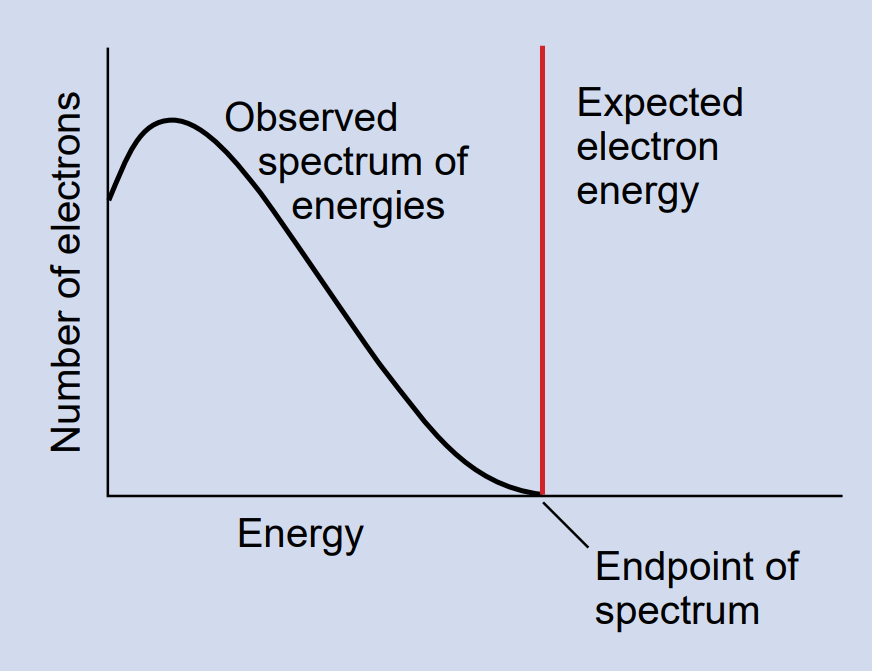
\includegraphics[width=0.5\textwidth]{Immagini/Spettro Beta 2.png}
    \caption{Esempio di spettro energetico degli elettroni emessi dai decadimenti $\beta$.}
    \label{Fig:Spettro Beta}
\end{figure}
L'ipotesi di decadimento in due corpi non conserva neanche lo spin. Il fatto che il decadimento $\beta$ sembrasse comportare tutte queste violazioni fu una temporanea crisi della fisica moderna. Per riuscire ad abbandonare questo mondo senza conservazione dell'energia, nel 1930 Wolfgang Pauli ipotizzò, con un ''rimedio disperato'', così definito nella lettera ai colleghi Radioattivi \cite{Pauli:1930pc}, che il decadimento in questione fosse in realtà un processo a tre corpi caratterizzato dalla presenza di una nuova particella inizialmente considerata impossibile da rivelare: il neutrino. La conservazione della carica elettrica richiede che quest'ultima sia una particella elettricamente neutra come i neutroni e i fotoni. Oltre a questo, la nuova particella deve avere una massa molto più piccola rispetto alla massa dell'elettrone in quanto l'end-point mostrato nella Figura \ref{Fig:Spettro Beta} corrisponde proprio al Q valore della reazione.  Infine il neutrino, come accennato prima, risolve anche la violazione della conservazione del momento angolare che si verificherebbe in sua assenza in quanto è un fermione di spin $\frac{1}{2}$ \cite{alma991008496889706031}.
Dalla prima ipotesi dell'esistenza del neutrino venne poi formulata da Fermi nel 1934 \cite{Fermi:1934hr} una teoria per formalizzare il decadimento $\beta$ che si può manifestare secondo le due reazioni:
\begin{equation}
    \text{Decadimento } \beta^-: \quad \ce{^A_ZX}\longrightarrow \ce{^A_{Z+1}Y}\,+\,e^-+\Bar{\nu}_e
    \label{eq:decadimento beta -}
\end{equation}
\begin{equation}
    \text{Decadimento } \beta^+: \quad \ce{^A_ZX}\longrightarrow \ce{^A_{Z-1}Y}\,+\,e^++\nu_e
\end{equation}
è qui possibile osservare la presenza di un positrone indicato con $e^+$ e dell'antineutrino elettronico indicato con $\Bar{\nu}_e$. 

Il neutrino, per sua natura, interagisce raramente con la materia, essendo un leptone che partecipa esclusivamente all’interazione debole e possiede una sezione d'urto estremamente ridotta. La sua esistenza rimase priva di conferme sperimentali per quasi vent’anni.
\section{Verifica sperimentale dell'esistenza del neutrino: esperimento di Reines e Cowan}
Nel 1944 Frederick Reines entrò nella Divisione Teorica a Los Alamos per il progetto Manhattan. Dopo lo scoppio della prima bomba atomica ci furono ulteriori esperimenti in cui si verificarono enormi flussi di radiazione gamma e neutroni. Il gruppo di Reines, grazie alla teoria del decadimento $\beta$ di Fermi, ipotizzò la presenza di un grande flusso di antineutrini generato dalle serie di decadimenti $\beta^-$ che seguono la fissione nucleare all'interno della bomba. Si pensò così di sfruttare questo enorme flusso per compensare la minuscola sezione d'urto dei neutrini, dal momento che interagiscono solamente attraverso interazioni deboli.
\\Nel 1951 Frederick Reines e Clyde Cowan diedero inizio al progetto Poltergeist, il primo esperimento sulla fisica del neutrino \cite{Reines:1997bk}. 
Tuttavia, solamente nel 1956, con l'esperimento di Savannah River si ebbe l'evidenza sperimentale dell'esistenza del neutrino.
In questo esperimento fu utilizzato il primo reattore nucleare per uso civile, ideato da Enrico Fermi, come sorgente di neutrini in quanto fra i prodotti della fissione ci sono emettitori $\beta$ a vita media breve. L'apparato sperimentale consiste in un serbatorio di soluzione acquosa di $\ce{CdCl_2}$ circondato da due scintillatori liquidi, come rappresentato schematicamente in Figura \ref{Fig:Apparato sperimentale R&C}.\\ Il rate di interazione può essere espresso nel seguente modo:
\begin{equation}
    R=\frac{\Delta n}{\Delta t}=\Phi_\nu\cdot N_T\cdot\sigma
    \label{eq:intsec}
\end{equation}
dove $\Phi_\nu$ rappresenta il flusso di neutrini, $N_T$ il numero di bersagli e $\sigma$ la sezione d'urto dell'interazione che dipende dalla reazione considerata. Reines e Cowan hanno potuto bilanciare la piccola sezione d'urto ($\sigma$) del (anti)neutrino nella relazione \ref{eq:intsec} sfruttando il consistente flusso ($\Phi_\nu$) proveniente dai prodotti di fissione e, sopratutto, sfruttando l'enorme quantità di idrogeno ($N_T$) presenti all'interno dei $200$ litri di soluzione acquosa.
\begin{figure}[ht]
    \centering
    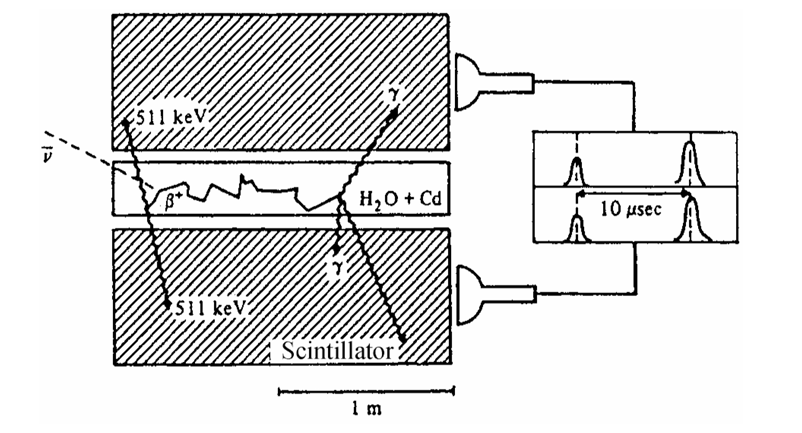
\includegraphics[width=0.8\textwidth]{Immagini/Apparato sperimentale R&C.png}
    \caption{Rappresentazione schematica dell'apparato sperimentale per la rivelazione dei neutrini usata da Reines e Cowan.}
    \label{Fig:Apparato sperimentale R&C}
\end{figure}
La reazione sfruttata in questo esperimento si basa sul decadimento $\beta$ inverso (IBD), che consiste nell'interazione tra un antineutrino elettronico e un protone, formando così un positrone e un neutrone:
\begin{equation}
    \Bar{\nu}_e+p\,\longrightarrow\,e^++n
    \label{eq:Beta inverso}
\end{equation}
i due prodotti sono essenziali per la misura di coincidenza ritardata. Il positrone, dopo aver perso energia, si annichila a riposo con un elettrone presente nella materia. Questo processo produce due fotoni da $511\,\unit{keV}$ ciascuno, emessi in direzioni opposte (back-to-back), in un tempo dell'ordine di $\sim$$\unit{ns}$ o inferiore:
\begin{equation}
    e^++e^-\,\longrightarrow\,2\gamma\,\,\,\,(511\,\unit{keV})
\end{equation}
I fotoni interagiscono con i rivelatori e forniscono un primo segnale. Successivamente, dopo circa $10\,\mu\unit{s}$ viene rilevato un secondo segnale che corrisponde alla cattura neutronica del $n$ sul $\ce{Cd}$ che porta il nucleo stesso ad uno stato eccitato. Dopo qualche $\unit{ps}$ avviene una diseccitazione elettromagnetica tramite l'emissione di un fotone: 
\begin{equation}
    \ce{^{113}Cd}+n\,\longrightarrow\,\ce{^{114}Cd}^*\,\longrightarrow\,\ce{^{114}Cd}+\gamma
\end{equation}
questa segnatura temporale fornisce in modo univoco la prova della presenza di un antineutrino elettronico, quindi l'esistenza del neutrino, distinguendo i due segnali dal fondo \cite{alma991017639394506031}. 
\section{Il neutrino nel Modello Standard}
\label{sec:Modello Standard}
\begin{figure}[h]
    \centering
    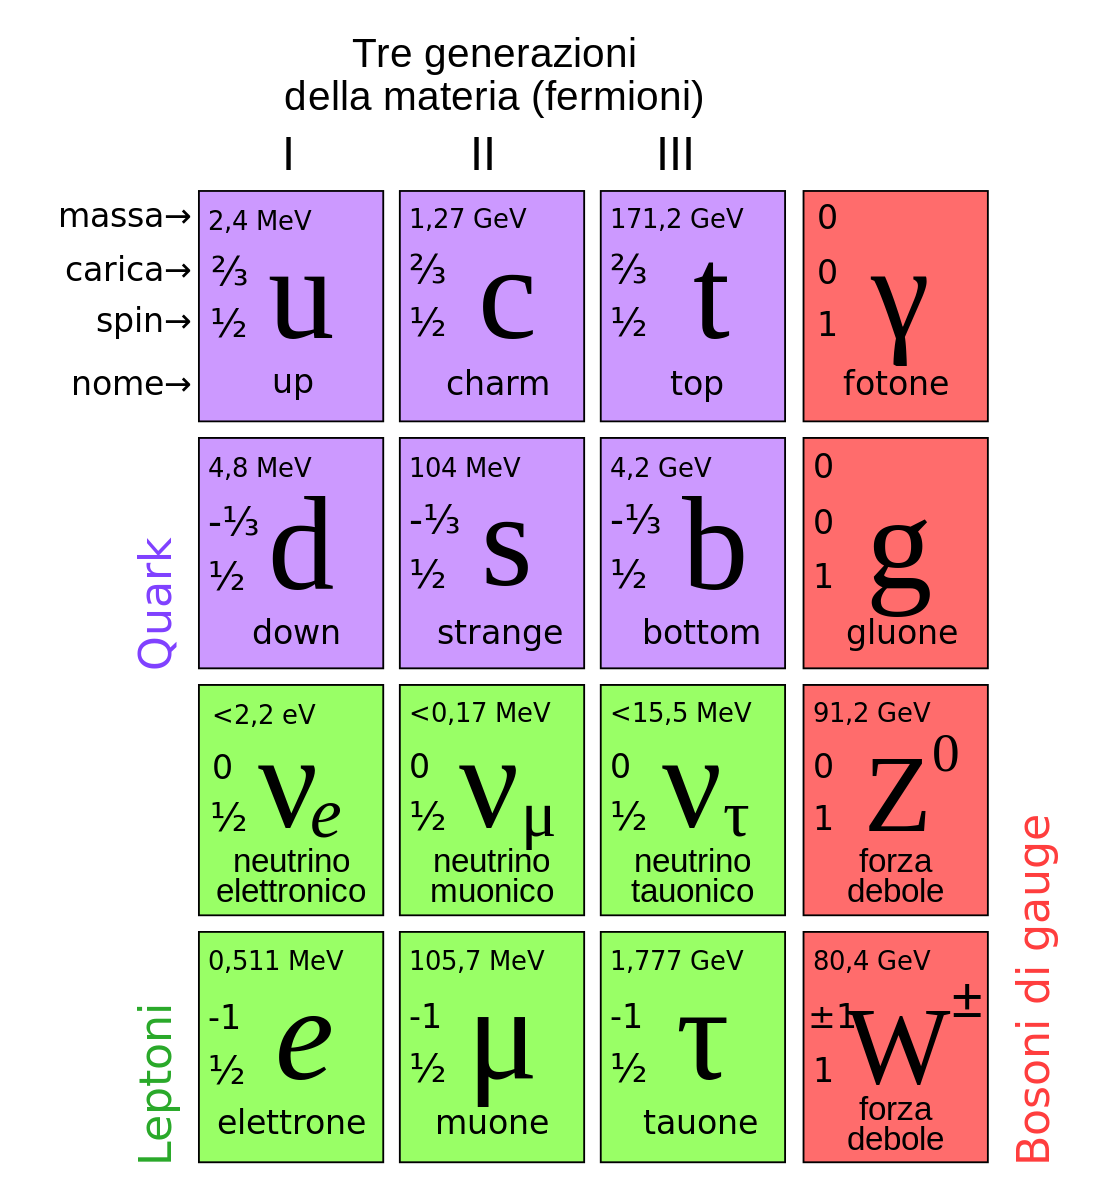
\includegraphics[width=0.6\textwidth]{Immagini/Modello Standard 2.png}
    \caption{Schema delle particelle del Modello Standard in cui sono stati inseriti i valori di massa, carica e spin. I quark e i leptoni sono presenti anche nella forma di antiparticella in cui le cariche sono opposte.}
    \label{Fig:Modello Standard}
\end{figure}
Un aspetto chiave per comprendere le proprietà principali dei neutrini è capire come essi siano inseriti all'interno del Modello Standard delle particelle elementari. Questo modello descrive e unifica tre delle forze fondamentali: l'interazione elettromagnetica, l'interazione debole e l'interazione forte. Come è possibile osservare nella Figura \ref{Fig:Modello Standard}, le particelle elementari sono divise in famiglie: i quark, i leptoni e i bosoni. I quark e i leptoni sono fermioni e costituiscono la materia ordinaria; i bosoni sono le particelle mediatrici delle interazioni. 
Il neutrino, in particolare, si colloca nel Modello Standard come leptone insieme all'elettrone ($e$), al muone ($\mu$), al tauone ($\tau$) e alle relative antiparticelle. A differenza degli altri leptoni, che possono interagire sia attraverso l'interazione debole sia elettromagnetica, il neutrino interagisce solo attraverso la prima in quanto elettricamente neutro e esiste in tre sapori: elettronico ($\nu_e$), muonico ($\nu_\mu$) e tauonico ($\nu_\tau$), in associazione con i tre leptoni generati (o assorbiti) quando avviene un'interazione. Nel modello standard i neutrini sono privi di massa, ma le osservazioni delle oscillazioni provano il contrario.
\section{L'invisibilità dei neutrini}
I neutrini, come precisato nella sezione dedicata, sono le uniche particelle del Modello Standard che interagiscono solo tramite l'interazione nucleare debole. Sono particelle che quindi interagiscono debolmente con la materia: la stessa Terra risulta quasi trasparente al passaggio di queste particelle. Per stimare il rate di interazione è possibile usare la relazione \ref{eq:intsec}. La sezione d'urto dipende dell'interazione considerata e può variare tra $10^{-40}\,\unit{cm}^2$ e $10^{-45}\,\unit{cm}^2$. Il Modello Solare Standard, di cui parlerò nella sezione successiva, prevede un rate di neutrini totali di circa $2\cdot10^{38}\,\frac{\nu}{\unit{s}}$ da cui si può stimare un flusso sulla superficie terrestre di circa $\Phi_n\sim6\cdot10^{10}\,\frac{\nu}{\unit{cm}^2\cdot \unit{s}}$. Considerando una sezione d'urto di $10^{-45}\,\unit{cm^2}$ si può calcolare che per avere un singolo evento al giorno sono necessari circa $N_T=10^{30}$ target. Il flusso di neutrini non è quindi sufficiente a bilanciare la piccola sezione d'urto che caratterizza i processi di rivelazione. Bisogna poi considerare che molti dei primi esperimenti fatti, come esporrò nella prossima sezione, hanno una soglia di reazione che esclude la maggior parte dei neutrini che provengono dalla reazione protone-protone ($pp$). Per questo motivo, i rivelatori che caratterizzano gli esperimenti sui neutrini, per bilanciare la relazione \ref{eq:intsec}, sono composti da grandi masse. Bisogna infine considerare il fatto che la grande elusività dei neutrini se da un lato costituisce un grande problema dal punto di vista sperimentale, dall'altro fa sì che questi possano propagarsi senza subire deflessioni o rallentamenti,  consentendo di non perdere informazioni sulla loro direzionalità.


I rivelatori utilizzati in tutti gli esperimenti che descriverò non sono solo sensibili ai vari flussi di neutrini, ma a tutta la radiazione naturale che può interagire e creare un fondo nelle misure. La radiazione naturale, a cui anche noi siamo sottoposti è indotta principalmente dai raggi cosmici, dalla radioattività di tutto ciò che circonda il rivelatore e dal rivelatore stesso. I raggi cosmici sono delle particelle che colpiscono l'atmosfera terrestre con un rate che corrisponde a circa $1000\,\frac{1}{\unit{m}^2\cdot s}$. Queste particelle, accellerate da processi astrofisici, sono principalmente protoni per circa il $90\%$ e per il $9\%$ particelle $\alpha$, mentre il resto è composto da nuclei più pesanti. Tali particelle interagiscono nella parte alta dell'atmosfera terrestre, producendo sciami di particelle formate principalmente da adroni, muoni e neutrini \cite{Gaisser_Engel_Resconi_2016}. Per questo motivo, tipicamente, gli esperimenti sui neutrini vengono effettuati in profondità nel sottosuolo, così da sfruttare tutta la materia che circonda il rivelatore come schermo naturale. D'altra parte però, essendo esperimenti condotti in profondità, il rivelatore viene sottoposto ad una forte radiazione dovuta alla radioattività delle rocce circostanti. A costituire il fondo sono i prodotti di decadimento delle catene del $\ce{^{238}U}$ e del $\ce{^{232}Th}$. Oltre a queste due catene contribuiscono anche il $\ce{^{222}Rn}$, il $\ce{^{14}C}$  (anche presente negli anelli benzenici dei liquidi scintillanti) e il $\ce{^{40}K}$. Sotto questo punto di vista si cerca quindi, attraverso diverse tecniche, di lavorare con materiali ad alta radiopurezza per ridurre al minimo i segnali di fondo.
\section{Sorgenti di neutrini}
\label{sec:sorge}
I neutrini possono essere di origine naturale o artificiale e la produzione può essere spontanea o indotta dalla collisione di particelle.
 \begin{figure}[ht]
    \centering
    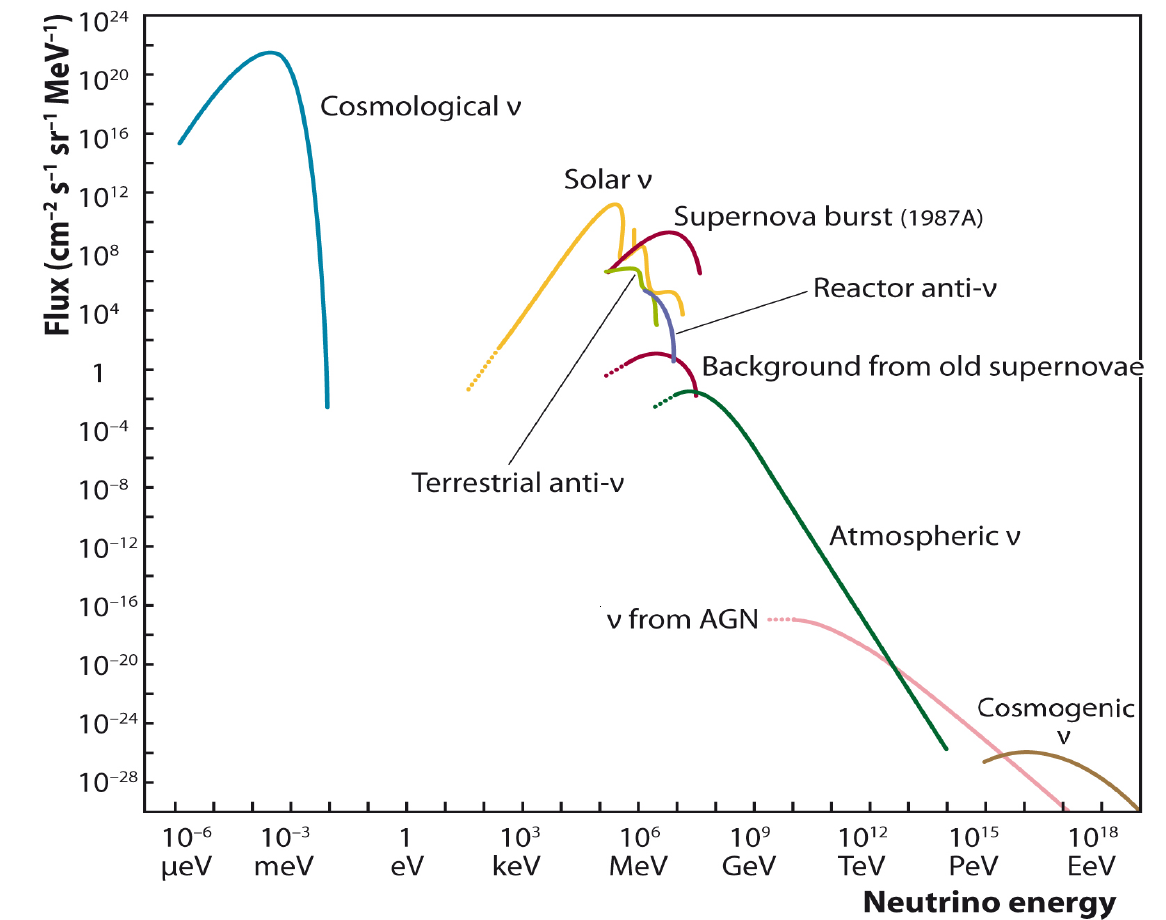
\includegraphics[width=0.8\textwidth]{Immagini/all_neutrino_fluxes.png}
    \caption{Flusso di tutti i tipi di neutrini originati da diverse sorgenti che raggiungono la Terra in funzione dell'energia \cite{Spiering:2012xe}.}
    \label{Fig:Flusso all neutrino}
\end{figure}
I neutrini generati artificialmente possono essere classificati in due principali processi: da reattore e da acceleratore. Invece, i neutrini di origine naturale, come illustrato nella Figura \ref{Fig:Flusso all neutrino}, vengono classificati in diversi modi. I neutrini meno energetici, ma con un flusso maggiore, sono di origine cosmologica \cite{Hannestad:2009xu} e costituiscono il C$\nu$B (Cosmic Neutrino Background) originata nei primi istanti di vita dell'Universo. Questi neutrini sono molto difficili da rivelare a causa della loro energia caratteristica di solo qualche $\unit{meV}$ e una sezione d'urto pari a circa $10^{-60}\,\unit{cm}^2$. Per questo motivo la rivelazione diretta rimane ancora un obiettivo tanto importante quanto complesso.
 
 
 Tra le sorgenti naturali, dopo i neutrini cosmologici, al crescere dell'energia, si trovano i neutrini solari \ref{sec:sole}, con un'energia caratteristica che va da qualche $\unit{keV}$ a qualche $\unit{MeV}$ di cui approfondirò nella sezione successiva. La sorgente più vicina a noi è rappresentata dalla stessa Terra. Il nostro pianeta continene infatti molti elementi radioattivi come il $\ce{^{232}Th}$ e il $\ce{^{238}U}$ o elementi instabili come il $\ce{^{40}K}$ (ampiamente presenti nel mantello e nella crosta terrestre) che tra i prodotti di decadimento producono anti-neutrini elettronici come mostrato nella relazione \ref{eq:decadimento beta -}. 

I neutrini di origine naturale possono provenire anche dal collasso di una stella massiccia, ovvero una supernova. In questo evento astrofisico, viene rilasciata una quantità enorme di energia sotto forma di radiazione elettromagnetica, materia e antineutrini con un'energia dell'ordine di decine di $\unit{MeV}$. I primi (anti)neutrini da supernova osservati provenivano da SN1987a, esplosa nella Grande Nube di Magellano. Tuttavia, il numero di neutrini rivelati fu limitato, poiché all'epoca erano in funzione solo pochi rivelatori.
 
 Oltre ai neutrini provenienti dal Sole, contribuiscono in maniera considerevole i neutrini atmosferici \cite{alma991017639394506032}. Questi sono originati dall'interazione dei raggi cosmici primari con la parte alta dell'atmosfera terrestre e hanno energia che può variare da circa $100\,\unit{MeV}$ fino a $100\,\unit{GeV}$. Da queste collisioni vengono prodotti sciami adronici che contengono principalmente mesoni (la maggior parte sono pioni) che decadono prima di raggiungere la superficie terrestre:
 \begin{equation}\label{eq:sciami}
\begin{gathered}
\pi^+\,\rightarrow\,\mu^++\nu_\mu \qquad\qquad  \mu^+\,\rightarrow \, e^++\nu_e+\Bar{\nu}_\mu\\
\pi^-\,\rightarrow\,\mu^-+\nu_\mu \qquad\qquad \mu^-\,\rightarrow \, e^-+\Bar{\nu}_e+\nu_\mu
\end{gathered}
\end{equation}
Dallo studio del flusso di neutrini muonici ed elettronici ci fu un problema completamente analogo al flusso di neutrini solari esposto nella sezione successiva. Infatti, il rapporto tra il numero di $\nu_\mu$ e $\nu_e$ è diverso da quello atteso. Il problema fu risolto da SuperKamiokaNDE \cite{Super-Kamiokande:1998kpq} nel 1998 che dimostrò l'accordo del contributo al flusso di neutrini elettronici ma un disaccordo nella componente muonica, spiegabile solamente con l'oscillazione in neutrini $\tau$. Questi risultati misero in evidenza la dipendenza del processo di oscillazione dalla distanza percorsa dai neutrini. 


Di origine astrofisica sono stati osservati neutrini di energia dell'ordine del $\unit{PeV}$ dall'esperimento IceCube \cite{Gaisser:2014foa}. Questi neutrini ad altissima energia possono essere stati originati da AGN (Active Galactic Nuclei) e da GRBs (Gamma-ray Bursts).
\section{Il problema dei neutrini solari}
\label{sec:sole}
Il Sole rappresenta la sorgente di neutrini più studiata e storicamente più importante. Oltre a produrre buona parte dei neutrini rivelabili sulla superficie terrestre, il Sole ha avuto un'importante collocazione storica sullo studio dei processi che alimentano le stelle e sulle proprietà fondamentali dei neutrini. I neutrini si formano all'interno del Sole attraverso processi termonucleari che producono energia sufficiente ad alimentare la sua stessa vita. Esistono due principali catene di reazione: la catena protone-protone ($pp$)  e il ciclo CNO (Carbonio, Azoto, Ossigeno). Queste corrispondono rispettivamente a circa il $99\%$ e al $1\%$ della potenza solare prodotta. I processi di fusione nucleare nel Sole producono nuclei di deuterio ($\ce{^2H}$) che a loro volta permettono la formazione dei neutroni necessari per costruire nuclei più pesanti, rilasciando una notevole quantità di energia. In queste reazioni si possono generare atomi di elio ($\ce{He}$) o, in misura minore, nuclei più pesanti coinvolti nel ciclo CNO. L'effetto netto è sempre: 
\begin{equation}
4p\,\longrightarrow\, \ce{^4He}+2e^++2\nu_e+26.3\,\unit{MeV}
\end{equation}
Ogni processo produce neutrini a diversa energia e quantità che vengono indicati in base al nome dei diversi prodotti di reazione:  $pp$$-\nu$, $\ce{^7Be}$$-\nu$, $pep$$-\nu$, $CNO$$-\nu$, $\ce{^8B}$$-\nu$ e $hep$$-\nu$.


Il Modello Solare Standard (SSM) \cite{Turck-Chièze_2016}, introdotto da John N. Bahcall nel 1962-1963 \cite{Bahcall:2002ng}, descrive l'evoluzione del Sole come oggetto astrofisico, consentendo di prevedere diverse grandezze chimiche e fisiche e la loro variazione nel tempo. Il SSM deriva dalla soluzione delle equazioni dell'evoluzione stellare, che descrivono come il Sole sia passato dalla sua formazione fino allo stato attuale. A partire dagli anni '80, il SSM ha subito significativi sviluppi, grazie all'affinamento delle misure sperimentali e alle osservazioni astrofisiche, inclusa l'eliosismologia. Queste tecniche hanno permesso di confrontare i dati osservativi con le previsioni del SSM, portando a un costante miglioramento del modello. La versione più aggiornata del SSM, nota come B16 \cite{Vinyoles:2018imb}, fornisce una previsione dettagliata delle proprietà del Sole, inclusi i flussi di neutrini prodotti in funzione dell'energia, come illustrato nella Figura \ref{Fig:Modello Solare Standard}. 
\begin{figure}[ht]
    \centering
    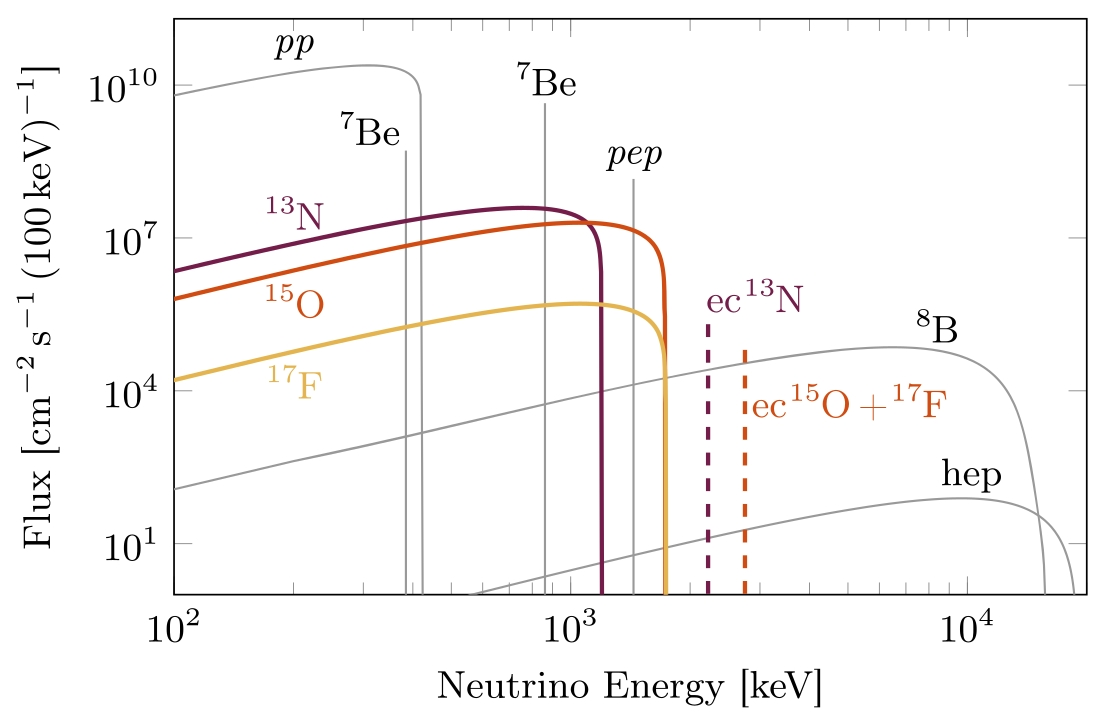
\includegraphics[width=0.85\textwidth]{Immagini/Modello Solare Standard 3.jpg}
    \caption{Flusso di neutrini solari previsto dal B16 al variare dell'energia \cite{BOREXINO:2020hox}.}
    \label{Fig:Modello Solare Standard}
\end{figure}


\subsection{Esperimenti sui neutrini solari}
In questa sezione vengono esaminati i principali sviluppi legati al problema dei neutrini solari e gli esperimenti chiave che hanno contribuito alla sua risoluzione \cite{Nakamura:2008zzk}.

\vspace{0,5cm}

\textbf{Homestake}\\
In contemporanea allo sviluppo del SSM, Raymond Davis e i suoi collaboratori svilupparono un primo esperimento per misurare il flusso di neutrini solari con Homestake \cite{Cleveland:1998nv}. Questo esperimento, costruito tra il 1965 e il 1967, aveva l'obiettivo di studiare il flusso di neutrini totali al di sopra di $0.814\,\unit{MeV}$, che rappresenta la soglia del processo adottato per osservare i singoli neutrini. Homestake prevedeva l'utilizzo di una tecnica radiochimica sfruttando il $\ce{^{37}Cl}$ nel processo di decadimento beta inverso \ref{eq:Beta inverso}:
\begin{equation}
    \nu_e+\ce{^{37}Cl}\,\longrightarrow\,\ce{^{37}Ar}+e^-
    \label{eq:Chlorine}
\end{equation}
come illustrato nella Figura \ref{Fig:Modello Solare Standard}, questo esperimento non sarebbe riuscito a rivelare i neutrini $pp$$-\nu$ perchè al di sotto della soglia di reazione. Risultava invece sensibile ai neutrini da reazioni $\ce{^7Be}$ e $\ce{^8B}$. Il rivelatore la cui massa di rivelazione era composta da $300\,\unit{ton}$ di tetracloroetilene ($\ce{C_2Cl_4}$), era situato in una miniera d'oro dismessa di Homestake in South Dakota per evitare il fondo dato dai raggi cosmici. La misura veniva effettuata estraendo e contando i singoli atomi di argon-37 formati dalla reazione \ref{eq:Chlorine}. La complessità di questa misura risiede sia nell'estrazione dei singoli atomi di argon in tutta la soluzione sia nel fatto che quest'ultimo ha una vita media di circa $35$ giorni. Raccogliendo dati per quasi 30 anni, Homestake riuscì ad osservare per la prima volta i neutrini solari, tuttavia i risultati ottenuti erano in contraddizione con i risultati teorici. Homestake misurò un rate di $2.56\,\unit{SNU}$\footnote{Il Solar Neutrino Unit (SNU) è una unità di misura per i flussi di neutrini. Corrisponde a $10^{-36}$ catture per atomo bersaglio per secondo.} che corrisponde a circa $1/3$ del rate previsto da SSM di $8.1\,\unit{SNU}$. Questa discrepanza diede inizio a quello che è conosciuto come ''il problema dei neutrini solari'', che non ebbe soluzione fino all'esperimento di SNO. 

\vspace{0,5cm}

\textbf{GALLEX (GNO)} \textbf{e SAGE}\\L'esperimento GALLEX, situato in Italia ai LNGS (Laboratori Nazionali del Gran Sasso), anch'esso di tipo radiochimico sfrutta il $\ce{^{71}Ga}$ nel decadimento $\beta$ inverso \ref{eq:Beta inverso}:
\begin{equation}
    \nu_e+\ce{^{71}Ga}\,\longrightarrow\,\ce{^{71}Ge}+e^-
    \label{eq:Gallex}
\end{equation}
il vantaggio del gallio come isotopo per la rivelazione risiede nell'energia di soglia della reazione che è di $233\,\unit{keV}$. Come si può valutare dalla figura \ref{Fig:Modello Solare Standard} in questo esperimento è possibile, per la prima volta, osservare parte dei neutrini provenienti dalla reazione $pp$. Nel 1998 GALLEX si è evoluto in GNO (Gallium Neutrino Observatory) ed ha continuato a prendere dati fino al 2003. Allo stesso modo SAGE, situato in Russia a Baksan ha acquisito dati utilizzando lo stesso identico processo di GALLEX. Entrambi gli esperimenti osservarono circa la metà del rate atteso, con un valore di $69.3\,\unit{SNU}$ per GALLEX (GNO) e un valore di $70.8\,\unit{SNU}$ per SAGE, contro il valore previsto da SSM di $126\,\unit{SNU}$. Questi dati sono quindi in contraddizione sia con la teoria che con i rate osservati da Homestake. 

La principale limitazione degli esperimenti di tipo radiochimico, oltre alle difficoltà già menzionate, è la capacità di fornire solo una stima del flusso totale dei neutrini, senza fornire informazioni sull'energia e sulla direzionalità. Questi aspetti sono cruciali per distinguere i contributi dei diversi neutrini e delle diverse sorgenti. Di conseguenza si sviluppò un secondo tipo di esperimento: gli esperimenti in tempo reale. Questo tipo di esperimento consente di rilevare i neutrini al momento dell'interazione, misurandone sia l'energia che la direzione di provenienza. Ciò è possibile grazie alla rilevazione delle particelle secondarie prodotte dall'interazione dei neutrini, attraverso fenomeni come la scintillazione o l'emissione di luce Cherenkov, registrate istantaneamente dai rivelatori.
\vspace{0,5cm}

\textbf{KamiokaNDE e Super-KamiokaNDE} \\
Nato per misurare la vita media del protone, KamiokaNDE (Kamioka Nucleon Decay Experiment) situato in Giappone, nella miniera di Kamioka, fu il primo esperimento sui neutrini in tempo reale. Successivamente potenziato e reso più massivo, Super-KamiokaNDE sfrutta $50\,\unit{kton}$ di acqua pura per rivelare i neutrini tramite scattering elastico:
\begin{equation}
    \nu_x+e^-\,\rightarrow\,\nu_x+e^-
    \label{eq:scattel}
\end{equation}
la relazione \ref{eq:scattel} fa riferimento alla possibilità dell'elettrone di interagire con un neutrino di sapore qualsiasi ($x=e,\mu,\tau$). Proprio in questo risiede il vantaggio degli esperimenti in tempo reale: le interazioni con i neutrini sono evidenziate attraverso la luce Cherenkov, prodotta dagli elettroni dallo scattering elastico. Questa luce viene poi catturata attraverso numerosi fotomoltiplicatori disposti sulla superficie interna in grado di trasformare e amplificare il segnale di luce in segnale elettrico. In questo modo, è possibile osservare i neutrini in tempo reale e ricavare la direzione di propagazione. Grazie allo studio della luce Cherenkov, a differenza dei precedenti esperimenti radiochimici, questo fu il primo esperimento che diede l'evidenza diretta che il Sole emette neutrini. A causa dell'alta soglia energetica di reazione (circa $7\,\unit{MeV}$ per KamiokaNDE e $5\,\unit{MeV}$ per Super-KamiokaNDE) questi esperimenti, facendo riferimento al SSM \ref{Fig:Modello Solare Standard}, osservano solo i neutrini $\ce{^8B}$$-\nu$ e $hep$$-\nu$, anche se quest'ultimi sono praticamente trascurabili.
   I risultati ottenuti sono nuovamente in contraddizione con il SSM e gli esperimenti precedenti confermando nuovamente il problema dei neutrini solari. La misura del flusso corrisponde a $2.35\cdot10^{6}\frac{\nu}{\unit{cm}^2\cdot \unit{s}}$, da confrontare con il valore atteso di $5.69\cdot10^{6}\frac{\nu}{\unit{cm}^2\cdot \unit{s}}$.


\vspace{0,5cm}

\textbf{SNO}\\
Il Sudbury Neutrino Observatory (SNO) \cite{SNO:2002ziz}, posto in una miniera attiva in Canada a $2000\,\unit{m}$ di profondità è composto da $1000\,\unit{ton}$ di acqua pesante ($\ce{D_2O}$) ultra-pura. La sostanziale differenza con (Super)KamiokaNDE risiede nel fatto che i neutrini possono interagire in tre diversi modi grazie alla presenza dell'atomo di deuterio:
\vspace{0.4cm}
\begin{itemize}
    \item \textbf{Scattering Elastico (ES)} con gli elettroni data dalla reazione \ref{eq:scattel} (come avviene in Super-KamiokaNDE). Tutti e tre i sapori di neutrino possono interagire in questo modo.
    \item \textbf{Correnti Cariche (CC)} sono le interazioni con il deutone:
    \begin{equation}
        \nu_e+d\,\rightarrow\,p+p+e^-
    \end{equation}
    e solamente i neutrini elettronici $\nu_e$ hanno accesso a questa reazione. Con una soglia di $1.4\,\unit{MeV}$.
    \item \textbf{Correnti Neutre (NC)} interazione di scattering con il deutone: 
    \begin{equation}
        \nu_x+d\,\rightarrow\,p+n+\nu_x
        \label{eq:NC}
    \end{equation}
    in cui tutti i neutrini attivi possono effettuare questa reazione con una soglia di $2.2\,\unit{MeV}$
\end{itemize}
Le soglie teoriche, però, nella pratica sono più elevate, intorno ai $4-5\,\unit{MeV}$, a causa della radioattività di fondo. L'esperimento SNO è concentrato a guardare solo neutrini provenienti da $\ce{^8B}$. Per la prima volta, il flusso totale misurato da SNO nel canale NC \ref{eq:NC} è in accordo con il Modello Solare Standard $\Phi_{NC}/\Phi_{SSM}\approx1$. Invece, la misura del flusso delle altre due reazioni nel canale unicamente elettronico erano inferiori rispetto al SSM. 
Dalla fisica standard del neutrino ci si aspettava che il flusso di correnti cariche misurato da SNO fosse uguale alle misura del flusso di scattering elastico da parte di Super-KamiokaNDE ($\Phi_{\text{SNO}}^{\text{CC}}(\nu_e)=\Phi_{\text{SK}}^{\text{ES}}(\nu_x)$), ma SNO diede una discrepanza tra i due valori maggiore di $3\sigma$, indicando indirettamente l'evidenza di  non $\nu_e$ all'interno del flusso di neutrini solari.

Super-KamiokaNDE, studiando i neutrini atmosferici (come descritto nella sezione \ref{sec:sorge}), e SNO, con i neutrini solari, hanno fornito le prime conferme sperimentali dell'oscillazione dei neutrini. Questo risultato fondamentale è valso il Premio Nobel per la Fisica nel 2015 a Takaaki Kajita e Arthur B. McDonald, per il loro contributo cruciale agli esperimenti che hanno dimostrato l'oscillazione dei neutrini.
\vspace{0,5cm}


\textbf{Borexino}\\
Situato nei LNGS, Borexino era anch'esso un esperimento in tempo reale ma, al posto di utilizzare acqua o acqua pesante, utilizzava un liquido scintillante. Il rivelatore, essendo molto più sensibile, permette di ridurre la quantità di liquido utilizzato e quindi di migliorare la radiopurezza di tutto l'apparato sperimentale. In questo modo è stato possibile osservare gran parte dello spettro energetico presente nella Figura \ref{Fig:Modello Solare Standard}, avendo una soglia di rivelazione di $0.19\,\unit{MeV}$. Nei vari anni in cui Borexino rimase attivo, si riuscì a studiare i neutrini provenienti dalla catena $pp$ \cite{BOREXINO:2014pcl} e successivamente dare la prima evidenza sperimentale dei neutrini provenienti da CNO \cite{BOREXINO:2020aww}. In aggiunta, Borexino diede un'ulteriore conferma diretta dell'oscillazione dei neutrini solari in tutto lo spettro energetico, individuando la correlazione tra questo nuovo fenomento e l'energia dei neutrini.
In questo modo si è risolto il problema dei neutrini solari mettendo in luce una nuova proprietà intrinseca del neutrino: l'oscillazione. 


Ricapitolando, diversi rivelatori e tecniche sperimentale riescono a misurare differenti flussi di neutrini e nessuno di questi è quello previsto dal Modello Solare Standard. La soluzione è nella natura stessa del neutrino: è l'unica particella, per ora osservata, che oscilla nei suoi vari sapori in quanto gli autostati di sapore e di massa non sono coincidenti. Da questi esperimenti è emerso che l'oscillazione dei neutrini dipende fortemente dall'energia.
\section{Oscillazione dei neutrini}
L'oscillazione dei neutrini è un fenomeno quantistico ipotizzato per la prima volta da Bruno Pontecorvo nel 1957. Questo processo rappresenta la chiave per risolvere il problema dei neutrini solari e atmosferici, una questione aperta per decenni e che ha trovato conferma sperimentale grazie agli esperimenti SNO, Super-KamiokaNDE e Borexino tra la fine degli anni '80 e l'inizio degli anni 2000. L'oscillazione implica che un neutrino possa cambiare sapore dal punto di generazione a quello di rivelazione a causa della sua propagazione nello spazio. Come spiegato nella sezione \ref{sec:Modello Standard}, nel Modello Standard i neutrini sono introdotti insieme ai propri leptoni e si formano durante le interazioni deboli:
\begin{equation}
    \left(\begin{array}{l} \nu_e \\ e \end{array}\right)\qquad \left(\begin{array}{l} \nu_\mu \\ \mu \end{array}\right)\qquad \left(\begin{array}{l} \nu_\tau \\ \tau \end{array}\right)
    \label{eq:neutrino}
\end{equation}
Al momento della produzione, i neutrini si trovano in uno dei tre autostati di sapore, ciascuno associato ai leptoni con cui vengono generati (o assorbiti), come mostrato nella relazione \ref{eq:neutrino}. L'ipotesi chiave del modello è che gli autostati di massa e di sapore non coincidano: l'oscillazione avviene perché i neutrini $\nu_e$, $\nu_\mu$ e $\nu_\tau$ non corrispondono a stati di massa definiti, ma sono combinazioni lineari di questi. Una caratteristica chiave è che ogni autostato di massa evolve nel tempo a velocità diverse; di conseguenza, la loro combinazione, cioè il sapore, varia nel tempo e nello spazio. Quindi, mentre durante la sua produzione il neutrino si trova in un autostato di sapore, durante la propagazione, invece, lo fa secondo il suo autostato di massa. Autostati di sapore e di massa sono legati da una matrice unitaria $3\times3$, chiamata matrice di mixing. Chiamata anche matrice di Pontecorvo-Maki-Nakagawa-Sakata (PMNS), essa permette il cambio di base attraverso una rotazione tra l'autostato di sapore e l'autostato di massa \cite{alma991014412219706031}:
\begin{equation}
    \left(\begin{array}{l} \nu_e\\\nu_\mu\\\nu_\tau
    \end{array}\right)=U^*\left(\begin{array}{l} \nu_1\\\nu_2\\\nu_3
    \end{array}\right)\quad \Rightarrow\quad\left|\nu_\alpha\right\rangle=\sum_{k=1}^{3}U^*_{\alpha k}\left|\nu_k\right\rangle
    \label{eq:mix}
\end{equation}
$\left|\nu_\alpha\right\rangle$ rappresenta i diversi autostati di sapore $\alpha: e$ (elettrone), $\mu$ (muone), $\tau$ (tauone). I $\left|\nu_k\right\rangle$ sono gli autostati di massa con $k=1,2,3$. Dalla relazione \ref{eq:mix} emerge che ogni autostato di massa non ha sapore definito e ogni autostato di sapore non ha massa definita. I coefficienti della matrice PMNS rappresentano le ampiezze di probabilità per il cambiamento di sapore dei neutrini:
\begin{equation}
    U_{\text{PMNS}}={\begin{pmatrix}1&0&0\\0&c_{23}&s_{23}\\0&-s_{23}&c_{23}\end{pmatrix}}{\begin{pmatrix}c_{13}&0&s_{13}e^{-i\delta }\\0&1&0\\-s_{13}e^{i\delta }&0&c_{13}\end{pmatrix}}{\begin{pmatrix}c_{12}&s_{12}&0\\-s_{12}&c_{12}&0\\0&0&1\end{pmatrix}}
    \label{eq:PMNS}
\end{equation}
in cui si possono individuare i coefficienti $c_{ij}=\cos{\theta_{ij}}$ e $s_{ij}=\sin{\theta_{ij}}$ che sono rispettivamente il coseno e il seno degli angoli di mixing ($\theta_{12}$, $ \theta_{23}$ e $\theta_{13}$), appartenenti all'intervallo $[0;\pi/2)$. Inoltre, si può notare che la matrice è parametrizzata dal prodotto di tre diverse matrici che rappresentano una diversa rotazione di coppie di autostati: rispettivamente 32, 31 e 21. Il termine di fase $\delta\in[0;2\pi)$ è introdotto nell'ipotesi in cui l'oscillazione violi la simmetria CP. Nel caso in cui fosse diverso da 0 e da $\pi$, si avrebbe la conferma della violazione di CP.
\subsection{Oscillazione dei neutrini nel vuoto}
Si prenda in esame un neutrino, che si forma al tempo $t=0$, nella posizione $\mathbf{x}=\underline{0}$ e in un autostato di sapore qualsiasi $\alpha$. Nel vuoto i neutrini si propagano secondo l'Hamiltoniana $\hat{H}$ di particella libera. Sapendo che i neutrini di massa sono autostati dell'Hamiltoniana, possiamo scrivere la seguente equazione:
\begin{equation}
\hat{H}_k\left|\nu_k\right\rangle=E_k\left|\nu_k\right\rangle \qquad E_k=\sqrt{\mathbf{ p}^2+m_k^2}
\label{eq:auto}
\end{equation}
con autovalore $E_k$ che rappresenta l'energia dei neutrini in unità naturali. Dal momento che i neutrini hanno una massa molto piccola ($<1\,\unit{eV}$), nel caso in cui non si abbia a che fare con neutrini del fondo cosmico si possono effettuare due principali approssimazioni: i neutrini considerati sono in regime ultra-relativistico
\begin{equation}
    m_k<<E_k\Rightarrow E_k\simeq|\mathbf{p}_k|+\frac{m_k^2}{2|\mathbf{p}_k|}
    \label{eq:ultra}
\end{equation}
Inoltre, si può assumere che i momenti dei neutrini siano uguali: $|\mathbf{p}_i|\simeq |\mathbf{p}_j|\equiv |\mathbf{p}|$ che, in regime ultrarelativistico, può essere considerato uguale all'energia totale $|\mathbf{p}|\simeq E$.
Ora è possibile scrivere l'equazione di Schr\"odinger per gli autostati di massa:

\begin{equation}
    \hat{H}_k\left|\nu_k(t)\right\rangle=i\hbar\frac{d}{dt}\left|\nu_k(t)\right\rangle
    \label{eq:sch}
\end{equation}
Le due relazioni \ref{eq:auto} e \ref{eq:sch} implicano che gli autostati di massa dei neutrini evolvono nel tempo come onde piane:
\begin{equation}
    \left|\nu_k(t)\right\rangle=e^{-iE_kt}\left|\nu_k(0)\right\rangle
\end{equation}
Di conseguenza, l'evoluzione temporale  degli autostati di sapore \ref{eq:mix} è:
\begin{equation}
     \left|\nu_\alpha(t)\right\rangle=\sum_{k=1}^3U^*_{\alpha k}e^{-iE_kt}\left|\nu_k(0)\right\rangle
\end{equation}
Ora, è possibile calcolare l'ampiezza di probabilità di osservare la transizione tra due autostati di sapore differenti $\nu_\alpha\to\nu_\beta$ data dal prodotto bra-ket dei due stati:
\begin{equation}
    A_{\nu_\alpha\to\nu_\beta}(t)=\left\langle\nu_\beta\right|\nu_\alpha(t)\rangle=\sum_{k=1}^{3}\sum_{j=1}^3U_{\alpha k}^*e^{-iE_kt}U_{\beta j}\left\langle\nu_j\right|\nu_k\rangle=\sum_{k=1}^3U_{\alpha k}^*U_{\beta k}e^{-iE_kt}
\end{equation}
Sfruttando l'ortonormalità della base, formata dagli autostati di massa: $\left\langle\nu_j\right|\nu_k\rangle=\delta_{jk}$ e calcolando il quadrato del valore assoluto dell'ampiezza, si ottiene la probabilità che questa transizione avvenga:
\begin{equation}
    P_{\nu_\alpha\to\nu_\beta}(t)=\left|A_{\nu_\alpha\to\nu_\beta}(t)\right|^2=\sum_{k,j}U_{\alpha k}^*U_{\beta k}U_{\alpha j}U_{\beta j}^*e^{-i(E_k-E_j)t}
\end{equation}
Per i neutrini ultra-relativistici, come mostrato nella relazione \ref{eq:ultra}, si può scrivere la differenza di energia in termini di differenza di massa:
\begin{equation}
    \Delta E_{kj}=E_k-E_j\simeq\frac{m^2_k-m^2_j}{2E}=\frac{\Delta m^2_{kj}}{2E}
\end{equation}
La probabilità diventa quindi:
\begin{equation}
     P_{\nu_\alpha\to\nu_\beta}(L, E)=\sum_{k,j}U_{\alpha k}^*U_{\beta k}U_{\alpha j}U_{\beta j}^*\exp{\left(-i\frac{\Delta m_{kj}^2L}{2E}\right)}
\end{equation}
%posso mettere nell'appendice come mai funziona questa approssimazione
I neutrini, trovandosi in regime ultra-relativistico, viaggiano a velocità prossime alla velocità della luce (nel vuoto). Quindi, è possibile approssimare $t\simeq L$, dove $L$ è la distanza percorsa dai neutrini. Sviluppando i calcoli, si può dimostrare che la probabilità che un neutrino di sapore iniziale $\alpha$ sia osservato con sapore $\beta$ è data da:
\begin{equation}
    \begin{aligned} P_{\nu_\alpha \rightarrow \nu_\beta}(L, E)=\delta_{\alpha \beta} & -4 \sum_{k>j} \Re \mathfrak{e}\left[U_{\alpha k}^* U_{\beta k} U_{\alpha j} U_{\beta j}^*\right] \sin ^2\left(\frac{\Delta m_{k j}^2 L}{4 E}\right) \\ & +2 \sum_{k>j} \Im \mathfrak{m}\left[U_{\alpha k}^* U_{\beta k} U_{\alpha j} U_{\beta j}^*\right] \sin \left(\frac{\Delta m_{k j}^2 L}{2 E}\right) .\end{aligned}
    \label{eq:tra}
\end{equation}
Questa espressione mette in luce come la probabilità di transizione sia funzione di due quantità sperimentali: la distanza sorgente-rivelatore e l'energia dei neutrini stessi. Invece, la frequenza di oscillazione dipende da $L$, $E$ e dalla differenza di massa $\Delta m_{kj}^2$. In questo modo si può indicare con $\Delta_{kj}$ la fase di oscillazione dei neutrini, ottenendo:
\begin{equation}
    \Delta_{kj}=\frac{\Delta m_{kj}^2L}{4E}
    \label{eq:osc}
\end{equation}
 Dalla fase di oscillazione si deduce che durante la propagazione, i neutrini oscillano tra i diversi sapori a causa della differenza nelle loro masse, che quindi devono essere necessariamente non nulle (almeno non tutte), contrariamente da quanto previsto dal Modello Standard.
 
 
 Una quantità importante è la lunghezza tipica di oscillazione, definita a partire dalla fase generata quando $\Delta _{kj}=2\pi$ e rappresenta la lunghezza tipica dopo la quale si ha un'oscillazione completa di una certa coppia di autostati di sapore:
\begin{equation}
    L_{kj}^{\text{osc}}=\frac{4\pi E}{\Delta m_{kj}^2}
\end{equation}
Applicando ora l'equazione \ref{eq:tra}, nel caso specifico in cui $\alpha=\beta$ cioè il sapore del neutrino iniziale e finale coincide, si parla di probabilità di sopravvivenza.  Questo caso è di particolare interesse per molti esperimenti attuali come JUNO. In analogia ai passaggi precedenti, con il modulo quadrato del prodotto tra il ket $\left|\nu_\alpha(t)\right\rangle$, come combinazione lineare degli autostati di massa evoluti nel tempo, sull'autostato di sapore $\left|\nu_\alpha\right\rangle$ si ottiene:
\begin{equation}
    P_{\nu_\alpha\to\nu_\alpha}=\left|\left\langle\nu_\alpha\right|\nu_\alpha(t)\right|^2
\end{equation}
nel caso specifico di JUNO, che rivela antineutrini elettronici, misurando quanti antineutrini rivelati con questo sapore vengono ritrovati con il medesimo sapore e che $P_{\nu_e\to\nu_e}=P_{\bar\nu_e\to\bar\nu_e}$ (dal teorema di conservazione di CPT) si può ottenere la probabilità di sopravvivenza nel seguente modo:
\begin{equation}
    \begin{aligned} P\left(\bar{\nu}_e \rightarrow \bar{\nu}_e\right)=1 & -\cos ^4\left(\theta_{13}\right) \sin ^2\left(2 \theta_{12}\right) \sin ^2\left(\Delta_{21}\right) \\ & -\cos ^2\left(\theta_{12}\right) \sin ^2\left(2 \theta_{13}\right) \sin ^2\left(\Delta_{31}\right) \\ & -\sin ^2\left(\theta_{12}\right) \sin ^2\left(2 \theta_{13}\right) \sin ^2\left(\Delta_{32}\right)\end{aligned}
    \label{eq:Prob}
\end{equation}
La probabilità di sopravvivenza, e quindi in generale la probabilità di oscillazione, dipende in particolare dagli angoli di mixing, dalla differenza tra i quadrati delle masse, dall'energia del neutrino e dalla sua distanza percorsa. I parametri misurabili in laboratorio, come detto in precedenza, sono il numero di eventi rispetto alla distanza $L$ e all'energia $E$, mentre i tre angoli di mixing ($\theta_{kj}$) e le tre differenze di masse al quadrato ($\Delta m_{jk}^2$) sono i sei parametri liberi. 

Le oscillazioni dei neutrini rappresentano la prima evidenza che queste particelle possiedono una massa diversa da zero, contrariamente a quanto previsto dal Modello Standard. Come emerge dalla fase di oscillazione \ref{eq:osc}, questo fenomeno, non potrebbero avvenire se tutte le masse dei neutrini fossero identiche o nulle. Quindi, la scoperta delle oscillazioni non solo ha risolto il problema dei neutrini solari e atmosferici, ma ha evidenziato la necessità di estendere il Modello Standard per includere la massa dei neutrini.
\section{Stato delle oscillazioni e ordinamento di massa dei neutrini}
Di fondamentale importanza per comprendere del tutto il processo di oscillazione dei neutrini risiede nel determinare quale sia il corretto ordinamento di massa. Attualmente, facendo riferimento ai più recenti risultati sperimentali \cite{esteban2024nufit60updatedglobalanalysis}, è noto che $\Delta m_{12}^2>0$ di conseguenza $m_2>m_1$. Il problema risiede nel segno di $\Delta m_{31}^2$ o analogamente $\Delta m_{32}^2$, che per semplicità sono indicati con la notazione $\Delta m_{3\ell}^2$ con $\ell=1,2$. Il segno di $\Delta m_{3\ell}^2$ determina due modi di riordinare le masse dei neutrini, come rappresentato in Figura \ref{Fig:Ordinamento}. 
 \begin{figure}[ht]
    \centering
    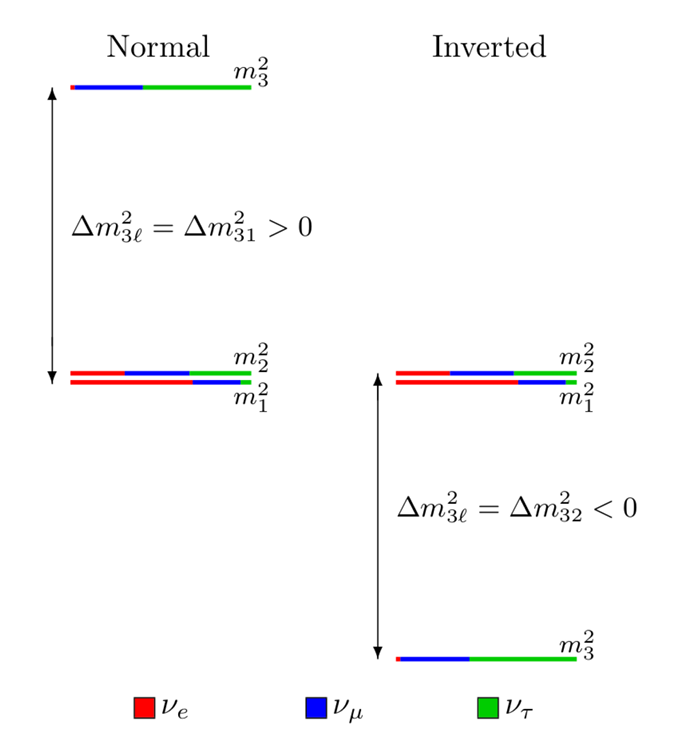
\includegraphics[width=0.6\textwidth]{Immagini/Ordinamento.png}
    \caption{Schema in cui sono rappresentati i due ordinamenti di massa del neutrino: normale e inverso. I colori rappresentano il fatto che ogni autostato di massa è combinazione lineare di autostati di sapore.}
    \label{Fig:Ordinamento}
\end{figure}
\begin{itemize}
    \item \textbf{Ordinamento Normale (NO):} $\Delta m_{3\ell}^2>0$ di conseguenza il terzo autostato di massa risulta maggiore rispetto ai primi due.
    \item \textbf{Ordinamento Inverso (IO):} $\Delta m_{3\ell}^2<0$ di conseguenza il terzo autostato è il più leggero.
\end{itemize}
Come si può notare dalla Figura \ref{Fig:Ordinamento}, la differenza di massa tra $\nu_1$ e $\nu_2$ è molto più piccola rispetto alla differenza di massa con $\nu_3$. Infatti $\Delta m_{21}^2=7.49\cdot10^{-5}\,\unit{eV^2}$ mentre $|\Delta m_{3\ell}|=2.51\cdot10^{-3}\,\unit{eV^2}$. Attualmente i valori di entrambi gli ordinamenti degli angoli di mixing, delle differenze di massa e del termine di fase $\delta_{CP}$, sono stati stimati attraverso fit globale sui dati provenienti da tutti gli esperimenti sulle oscillazioni di neutrini \cite{esteban2024nufit60updatedglobalanalysis}, aggiornato a settembre 2024, e sono riportati nella tabella \ref{tab:val}.
\begin{table}[h!]
\centering
\renewcommand{\arraystretch}{1.3}
\begin{tabular}{l @{\hspace{2cm}} l}
\toprule
\textbf{Parametri} & \textbf{NuFit-6.0 \cite{esteban2024nufit60updatedglobalanalysis} W SK-ATM} \\ 
\midrule
\textbf{NO} & \textbf{bfp $\pm 1\sigma$} \\ 
\midrule
$\sin^2 \theta_{12}$     & $0.308^{+0.012}_{-0.011}$ \\
$\sin^2 \theta_{23}$     & $0.470^{+0.017}_{-0.013}$ \\
$\sin^2 \theta_{13}$     & $0.02215^{+0.00056}_{-0.00058}$ \\
$\delta_{CP}/\circ$                     & $212^{+26}_{-41}$ \\
$\frac{\Delta m^2_{21}}{10^{-5} \text{eV}^2}$ & $7.49^{+0.19}_{-0.19}$ \\
$\frac{\Delta m^2_{3\ell}}{10^{-3} \text{eV}^2}$ & $2.513^{+0.021}_{-0.019}$ \\
\midrule
\textbf{IO} & \textbf{bfp $\pm 1\sigma$} \\ 
\midrule
$\sin^2 \theta_{12}$     & $0.308^{+0.012}_{-0.011}$ \\
$\sin^2 \theta_{23}$     & $0.550^{+0.012}_{-0.015}$ \\
$\sin^2 \theta_{13}$     & $0.02215^{+0.00056}_{-0.00058}$ \\
$\delta_{CP}/\circ$                     & $212^{+26}_{-41}$ \\
$\frac{\Delta m^2_{21}}{10^{-5} \text{eV}^2}$ & $7.49^{+0.19}_{-0.19}$ \\
$\frac{\Delta m^2_{3\ell}}{10^{-3} \text{eV}^2}$ & $-2.484^{+0.020}_{-0.020}$ \\
\bottomrule
\end{tabular}
\caption{Parametri di oscillazione dei tre sapori di neutrino ottenuti con un fit globale utilizzando anche i dati atmosferici e di SK. Oltre al Best Fit Point è indicata l'incertezza a $1\sigma$.}
\label{tab:val}
\end{table}
L'importanza di comprendere l'ordinamento di massa corretta e il valore di tutti i parametri elencati è legata alla presenza di molte grandi domande ancora aperte sulla fisica del neutrino. Come accennato in precedenza, il fattore di fase $\delta_{CP}$, presente nella matrice $U_{\text{PMNS}}$ \ref{eq:PMNS}, permette di studiare la possibile violazione della simmetria CP (coniugazione di carica e inversione delle coordinate spaziali) nel settore leptonico; questa potrebbe fornire l'ultima evidenza per spiegare l'assimetria presente tra materia e anti-materia nell'universo.

L'ordinamento di massa è anche fondamentale per dare indicazioni indirette sulla natura dei neutrini in quanto potrebbe determinare se i neutrini sono particelle di Majorana o particelle di Dirac. Le particelle di Dirac sono particelle diverse dalle proprie antiparticelle: nel caso dei neutrini i corrispondenti anti-neutrini avrebbero numero leptonico differente. Invece, se fossero particelle di Majorana, i neutrini e antineutrini avrebbero lo stesso numero leptonico.


Dal 1930, a partire dalla prima ipotesi teorica dell'esistenza del neutrino, sono stati fatti enormi progressi nella comprensione della fisica di questa particella. Dalla prima rivelazione fino alla soluzione del problema dei neutrini solari e atmosferici, molte domande hanno trovato risposta. Oggi, l'esperimento JUNO (Jiangmen Underground Neutrino Observatory) si inserisce in questo scenario con l'obiettivo di affrontare la più grande sfida ancora aperta nella fisica dei neutrini: l'ordinamento di massa.
\newpage